\documentclass[tikz,border=8pt]{standalone}
\usetikzlibrary{arrows.meta}
\begin{document}
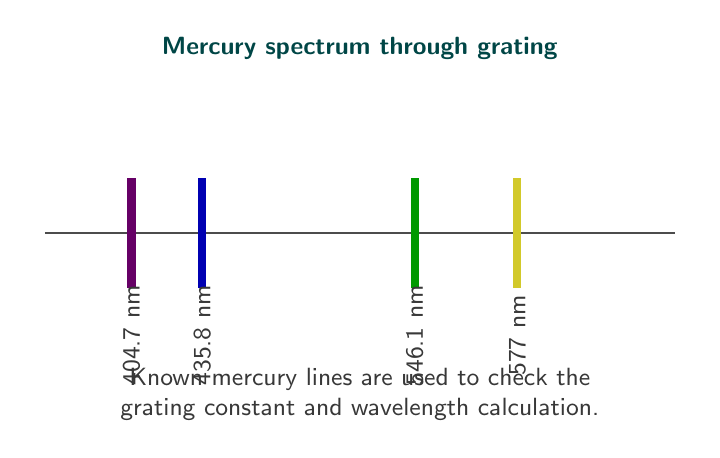
\begin{tikzpicture}[
  line/.style={draw=black!70,line width=0.75pt},
  label/.style={font=\sffamily\small,text=black!78},
  title/.style={font=\sffamily\bfseries\small,text=teal!55!black},
]
\node[title] at (0,2.35) {Mercury spectrum through grating};
\draw[line] (-4,0)--(4,0);
\foreach \x/\col/\lab in {-2.9/violet!80!black/404.7 nm,-2.0/blue!70!black/435.8 nm,0.7/green!60!black/546.1 nm,2.0/yellow!80!black/577 nm}{
  \draw[\col,line width=3pt] (\x,-0.7)--(\x,0.7);
  \node[label,rotate=90] at (\x,-1.3) {\lab};
}
\node[label,align=center,text width=8.2cm] at (0,-2.05)
  {Known mercury lines are used to check the grating constant and wavelength calculation.};
\end{tikzpicture}
\end{document}
